% Options for packages loaded elsewhere
% Options for packages loaded elsewhere
\PassOptionsToPackage{unicode}{hyperref}
\PassOptionsToPackage{hyphens}{url}
\PassOptionsToPackage{dvipsnames,svgnames,x11names}{xcolor}
%
\documentclass[
  number]{elsarticle}
\usepackage{xcolor}
\usepackage{amsmath,amssymb}
\setcounter{secnumdepth}{5}
\usepackage{iftex}
\ifPDFTeX
  \usepackage[T1]{fontenc}
  \usepackage[utf8]{inputenc}
  \usepackage{textcomp} % provide euro and other symbols
\else % if luatex or xetex
  \usepackage{unicode-math} % this also loads fontspec
  \defaultfontfeatures{Scale=MatchLowercase}
  \defaultfontfeatures[\rmfamily]{Ligatures=TeX,Scale=1}
\fi
\usepackage{lmodern}
\ifPDFTeX\else
  % xetex/luatex font selection
\fi
% Use upquote if available, for straight quotes in verbatim environments
\IfFileExists{upquote.sty}{\usepackage{upquote}}{}
\IfFileExists{microtype.sty}{% use microtype if available
  \usepackage[]{microtype}
  \UseMicrotypeSet[protrusion]{basicmath} % disable protrusion for tt fonts
}{}
\makeatletter
\@ifundefined{KOMAClassName}{% if non-KOMA class
  \IfFileExists{parskip.sty}{%
    \usepackage{parskip}
  }{% else
    \setlength{\parindent}{0pt}
    \setlength{\parskip}{6pt plus 2pt minus 1pt}}
}{% if KOMA class
  \KOMAoptions{parskip=half}}
\makeatother
% Make \paragraph and \subparagraph free-standing
\makeatletter
\ifx\paragraph\undefined\else
  \let\oldparagraph\paragraph
  \renewcommand{\paragraph}{
    \@ifstar
      \xxxParagraphStar
      \xxxParagraphNoStar
  }
  \newcommand{\xxxParagraphStar}[1]{\oldparagraph*{#1}\mbox{}}
  \newcommand{\xxxParagraphNoStar}[1]{\oldparagraph{#1}\mbox{}}
\fi
\ifx\subparagraph\undefined\else
  \let\oldsubparagraph\subparagraph
  \renewcommand{\subparagraph}{
    \@ifstar
      \xxxSubParagraphStar
      \xxxSubParagraphNoStar
  }
  \newcommand{\xxxSubParagraphStar}[1]{\oldsubparagraph*{#1}\mbox{}}
  \newcommand{\xxxSubParagraphNoStar}[1]{\oldsubparagraph{#1}\mbox{}}
\fi
\makeatother


\usepackage{longtable,booktabs,array}
\usepackage{calc} % for calculating minipage widths
% Correct order of tables after \paragraph or \subparagraph
\usepackage{etoolbox}
\makeatletter
\patchcmd\longtable{\par}{\if@noskipsec\mbox{}\fi\par}{}{}
\makeatother
% Allow footnotes in longtable head/foot
\IfFileExists{footnotehyper.sty}{\usepackage{footnotehyper}}{\usepackage{footnote}}
\makesavenoteenv{longtable}
\usepackage{graphicx}
\makeatletter
\newsavebox\pandoc@box
\newcommand*\pandocbounded[1]{% scales image to fit in text height/width
  \sbox\pandoc@box{#1}%
  \Gscale@div\@tempa{\textheight}{\dimexpr\ht\pandoc@box+\dp\pandoc@box\relax}%
  \Gscale@div\@tempb{\linewidth}{\wd\pandoc@box}%
  \ifdim\@tempb\p@<\@tempa\p@\let\@tempa\@tempb\fi% select the smaller of both
  \ifdim\@tempa\p@<\p@\scalebox{\@tempa}{\usebox\pandoc@box}%
  \else\usebox{\pandoc@box}%
  \fi%
}
% Set default figure placement to htbp
\def\fps@figure{htbp}
\makeatother





\setlength{\emergencystretch}{3em} % prevent overfull lines

\providecommand{\tightlist}{%
  \setlength{\itemsep}{0pt}\setlength{\parskip}{0pt}}



 
\usepackage[]{natbib}
\bibliographystyle{elsarticle-num}


\makeatletter
\@ifpackageloaded{caption}{}{\usepackage{caption}}
\AtBeginDocument{%
\ifdefined\contentsname
  \renewcommand*\contentsname{Table of contents}
\else
  \newcommand\contentsname{Table of contents}
\fi
\ifdefined\listfigurename
  \renewcommand*\listfigurename{List of Figures}
\else
  \newcommand\listfigurename{List of Figures}
\fi
\ifdefined\listtablename
  \renewcommand*\listtablename{List of Tables}
\else
  \newcommand\listtablename{List of Tables}
\fi
\ifdefined\figurename
  \renewcommand*\figurename{Figure}
\else
  \newcommand\figurename{Figure}
\fi
\ifdefined\tablename
  \renewcommand*\tablename{Table}
\else
  \newcommand\tablename{Table}
\fi
}
\@ifpackageloaded{float}{}{\usepackage{float}}
\floatstyle{ruled}
\@ifundefined{c@chapter}{\newfloat{codelisting}{h}{lop}}{\newfloat{codelisting}{h}{lop}[chapter]}
\floatname{codelisting}{Listing}
\newcommand*\listoflistings{\listof{codelisting}{List of Listings}}
\makeatother
\makeatletter
\makeatother
\makeatletter
\@ifpackageloaded{caption}{}{\usepackage{caption}}
\@ifpackageloaded{subcaption}{}{\usepackage{subcaption}}
\makeatother
\usepackage{bookmark}
\IfFileExists{xurl.sty}{\usepackage{xurl}}{} % add URL line breaks if available
\urlstyle{same}
\hypersetup{
  pdftitle={Marine Heatwaves in the Med Sea},
  pdfauthor={Simon Oiry; Maria Laura Zoffoli},
  pdfkeywords={Remote Sensing, Sentinel-2, Heatwaves},
  colorlinks=true,
  linkcolor={blue},
  filecolor={Maroon},
  citecolor={Blue},
  urlcolor={Blue},
  pdfcreator={LaTeX via pandoc}}


\setlength{\parindent}{6pt}
\begin{document}

\begin{frontmatter}
\title{Marine Heatwaves in the Med Sea \\\large{A temporale analysis} }
\author[1]{Simon Oiry%
\corref{cor1}%
}
 \ead{oirysimon@gmail.com} 
\author[2]{Maria Laura Zoffoli%
%
}


\affiliation[1]{organization={Nantes Université, UR 2160, F-44000
Nantes, France, Institut des Substances et Organismes de la Mer,
ISOMer},addressline={2 chemin de la
houssinière},city={Nantes},postcode={44300},postcodesep={}}
\affiliation[2]{organization={Consiglio Nazionale delle Ricerche,
Istituto di Scienze Marine (CNR-ISMAR), 00133 Rome,
Italy},,postcodesep={}}

\cortext[cor1]{Corresponding author}


        
\begin{abstract}
TBD
\end{abstract}





\begin{keyword}
    Remote Sensing \sep Sentinel-2 \sep 
    Heatwaves
\end{keyword}
\end{frontmatter}
    

Marine heatwaves (MHWs) are discrete and prolonged periods of
anomalously high sea temperatures that significantly exceed historical
baseline conditions. Specifically, a marine heatwave is generally
defined as an event lasting five or more consecutive days during which
sea temperatures exceed the 90th percentile threshold based on a 30-year
historical climatological period (Figure~\ref{fig-HW_explain}). These
events can vary in terms of duration, intensity, and spatial extent,
making a flexible yet rigorous approach necessary for accurate
characterization and comparison.

\phantomsection\label{cell-fig-HW_explain}
\begin{figure}[H]

\centering{

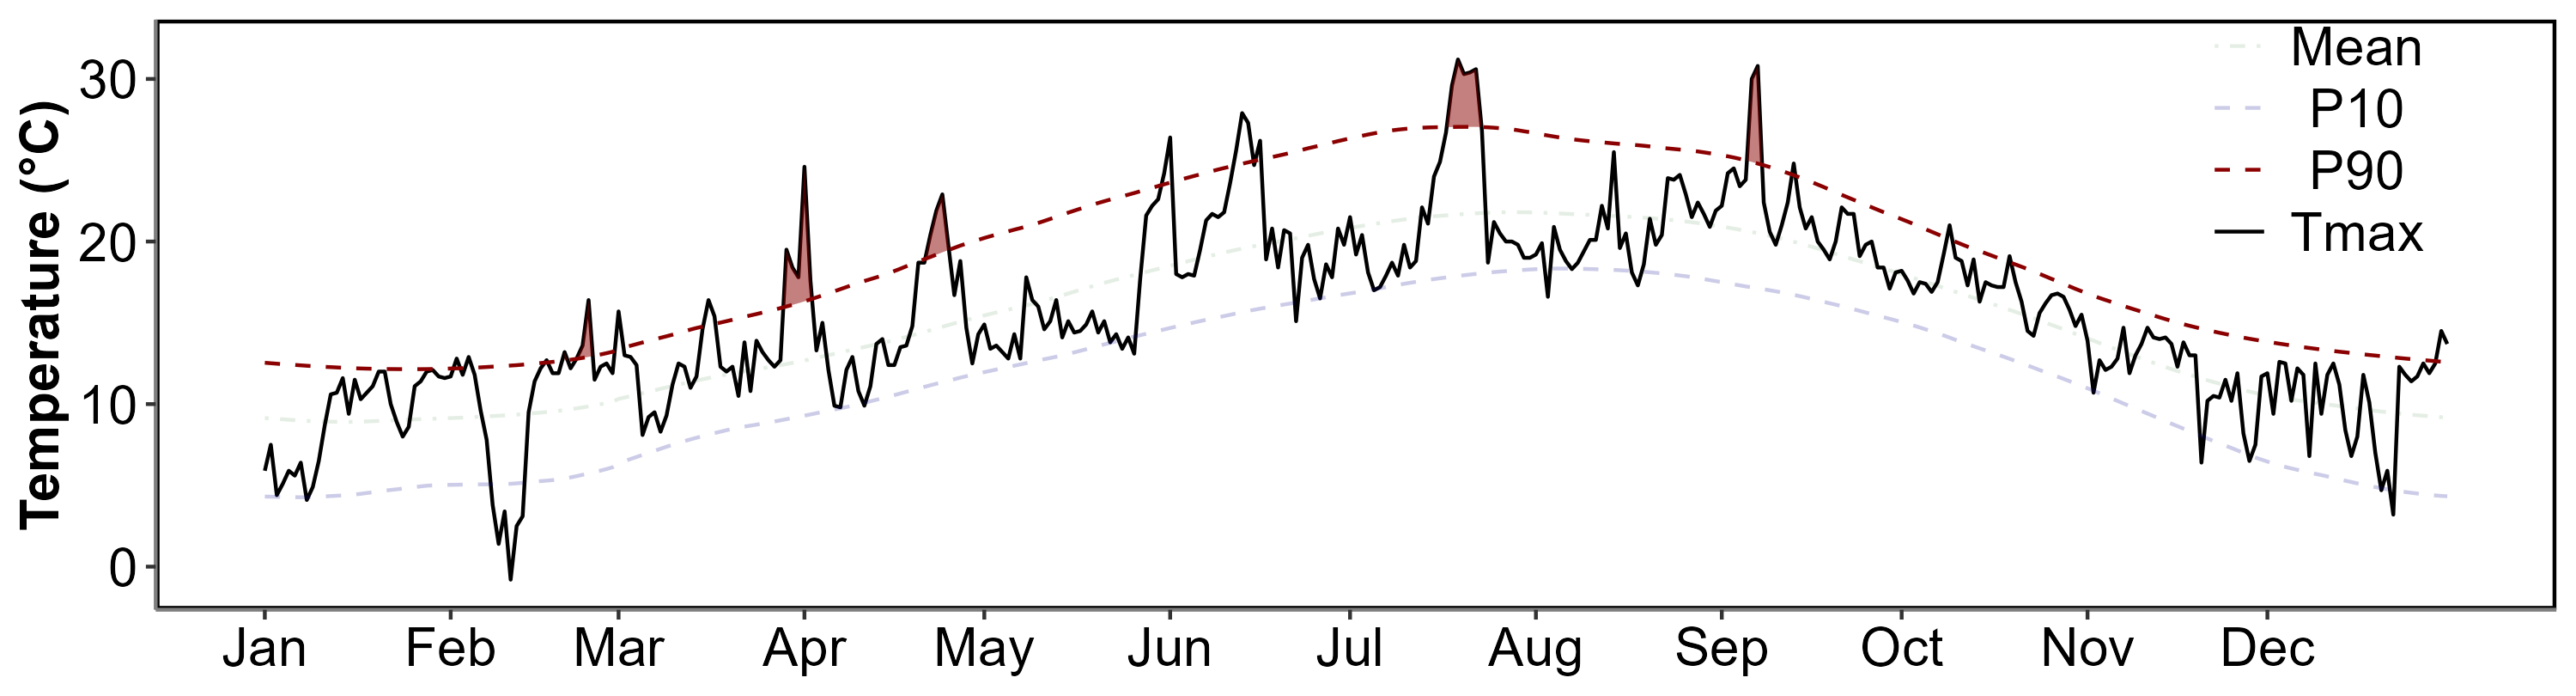
\includegraphics[width=1\linewidth,height=\textheight,keepaspectratio]{Figs/plot_Tmax_flame.png}

}

\caption{\label{fig-HW_explain}Exemple of heatwaves detection in
Quiberon France during the summer 2021}

\end{figure}%

The importance of studying marine heatwaves arises from their profound
ecological and socioeconomic impacts. They have been associated with
widespread disruptions to marine ecosystems, including shifts in species
distribution, local extinctions, significant mortality events, and
changes in primary productivity. Such ecological disturbances
subsequently affect fisheries, aquaculture, and biodiversity,
highlighting the broad-reaching implications of these events.

The Mediterranean Sea, characterized as a climate change hotspot, has
witnessed an increased frequency and intensity of marine heatwaves,
especially over recent decades. Mediterranean MHWs often coincide with
atmospheric heatwaves, further exacerbating their intensity and
ecological impacts. Concurrent atmospheric and marine heatwaves amplify
sea surface temperature anomalies, leading to intense ocean
stratification and extensive ecological disruption, including mass
mortalities of benthic invertebrates and seagrass decline.

In the Mediterranean, particularly in the Adriatic Sea, studies have
documented variable responses of primary productivity to MHW events. In
coastal and eutrophic regions, such as areas influenced by riverine
nutrient input, MHWs have resulted in increased phytoplankton biomass.
Conversely, offshore and oligotrophic regions typically exhibit reduced
chlorophyll-a concentrations during heatwaves, indicating a potential
decline in phytoplankton productivity. Such spatial heterogeneity
emphasizes the complexity of ecological responses and underscores the
importance of localized assessments.

Understanding marine heatwaves, particularly in sensitive regions like
the Mediterranean Sea, is crucial for developing informed management
strategies aimed at mitigating their ecological and socioeconomic
consequences. This necessity is heightened by projections indicating
further increases in MHW frequency, duration, and intensity, driven by
ongoing climate change.

\section{Methods}\label{methods}

Daily Sea Surface Temperature (SST) time series for the Mediterranean
Sea, spanning from 1982 onwards, were obtained from the Copernicus
Marine Environment Monitoring Service (CMEMS) platform
\citep{Copernicus_Sentinel, pisano2016new, embury2024satellite}.
Heatwave events were detected using the HeatwaveR package in R
\citep{heatwaveR}, adhering to the marine heatwave definition provided
by \citep{hobday2016hierarchical} and \citep{hobday2018categorizing}.

To establish a reference climatology, the first 30 years of the dataset
were utilized for each pixel within the Mediterranean Sea. Daily SST
values were subsequently compared against this baseline climatology. A
heatwave event was identified whenever the daily SST exceeded the 90th
percentile of the corresponding climatological distribution.
Additionally, consecutive events separated by fewer than two days were
merged and treated as a single continuous heatwave event.

Results are presented as annual maps of key heatwave metrics: the total
number of days classified as heatwave, the number of distinct heatwave
events, and the cumulative intensity of these events, defined as the sum
of daily SST exceedances above the climatological 90th percentile
threshold.

\phantomsection\label{cell-fig-MapMedSea}
\begin{figure}[H]

\centering{

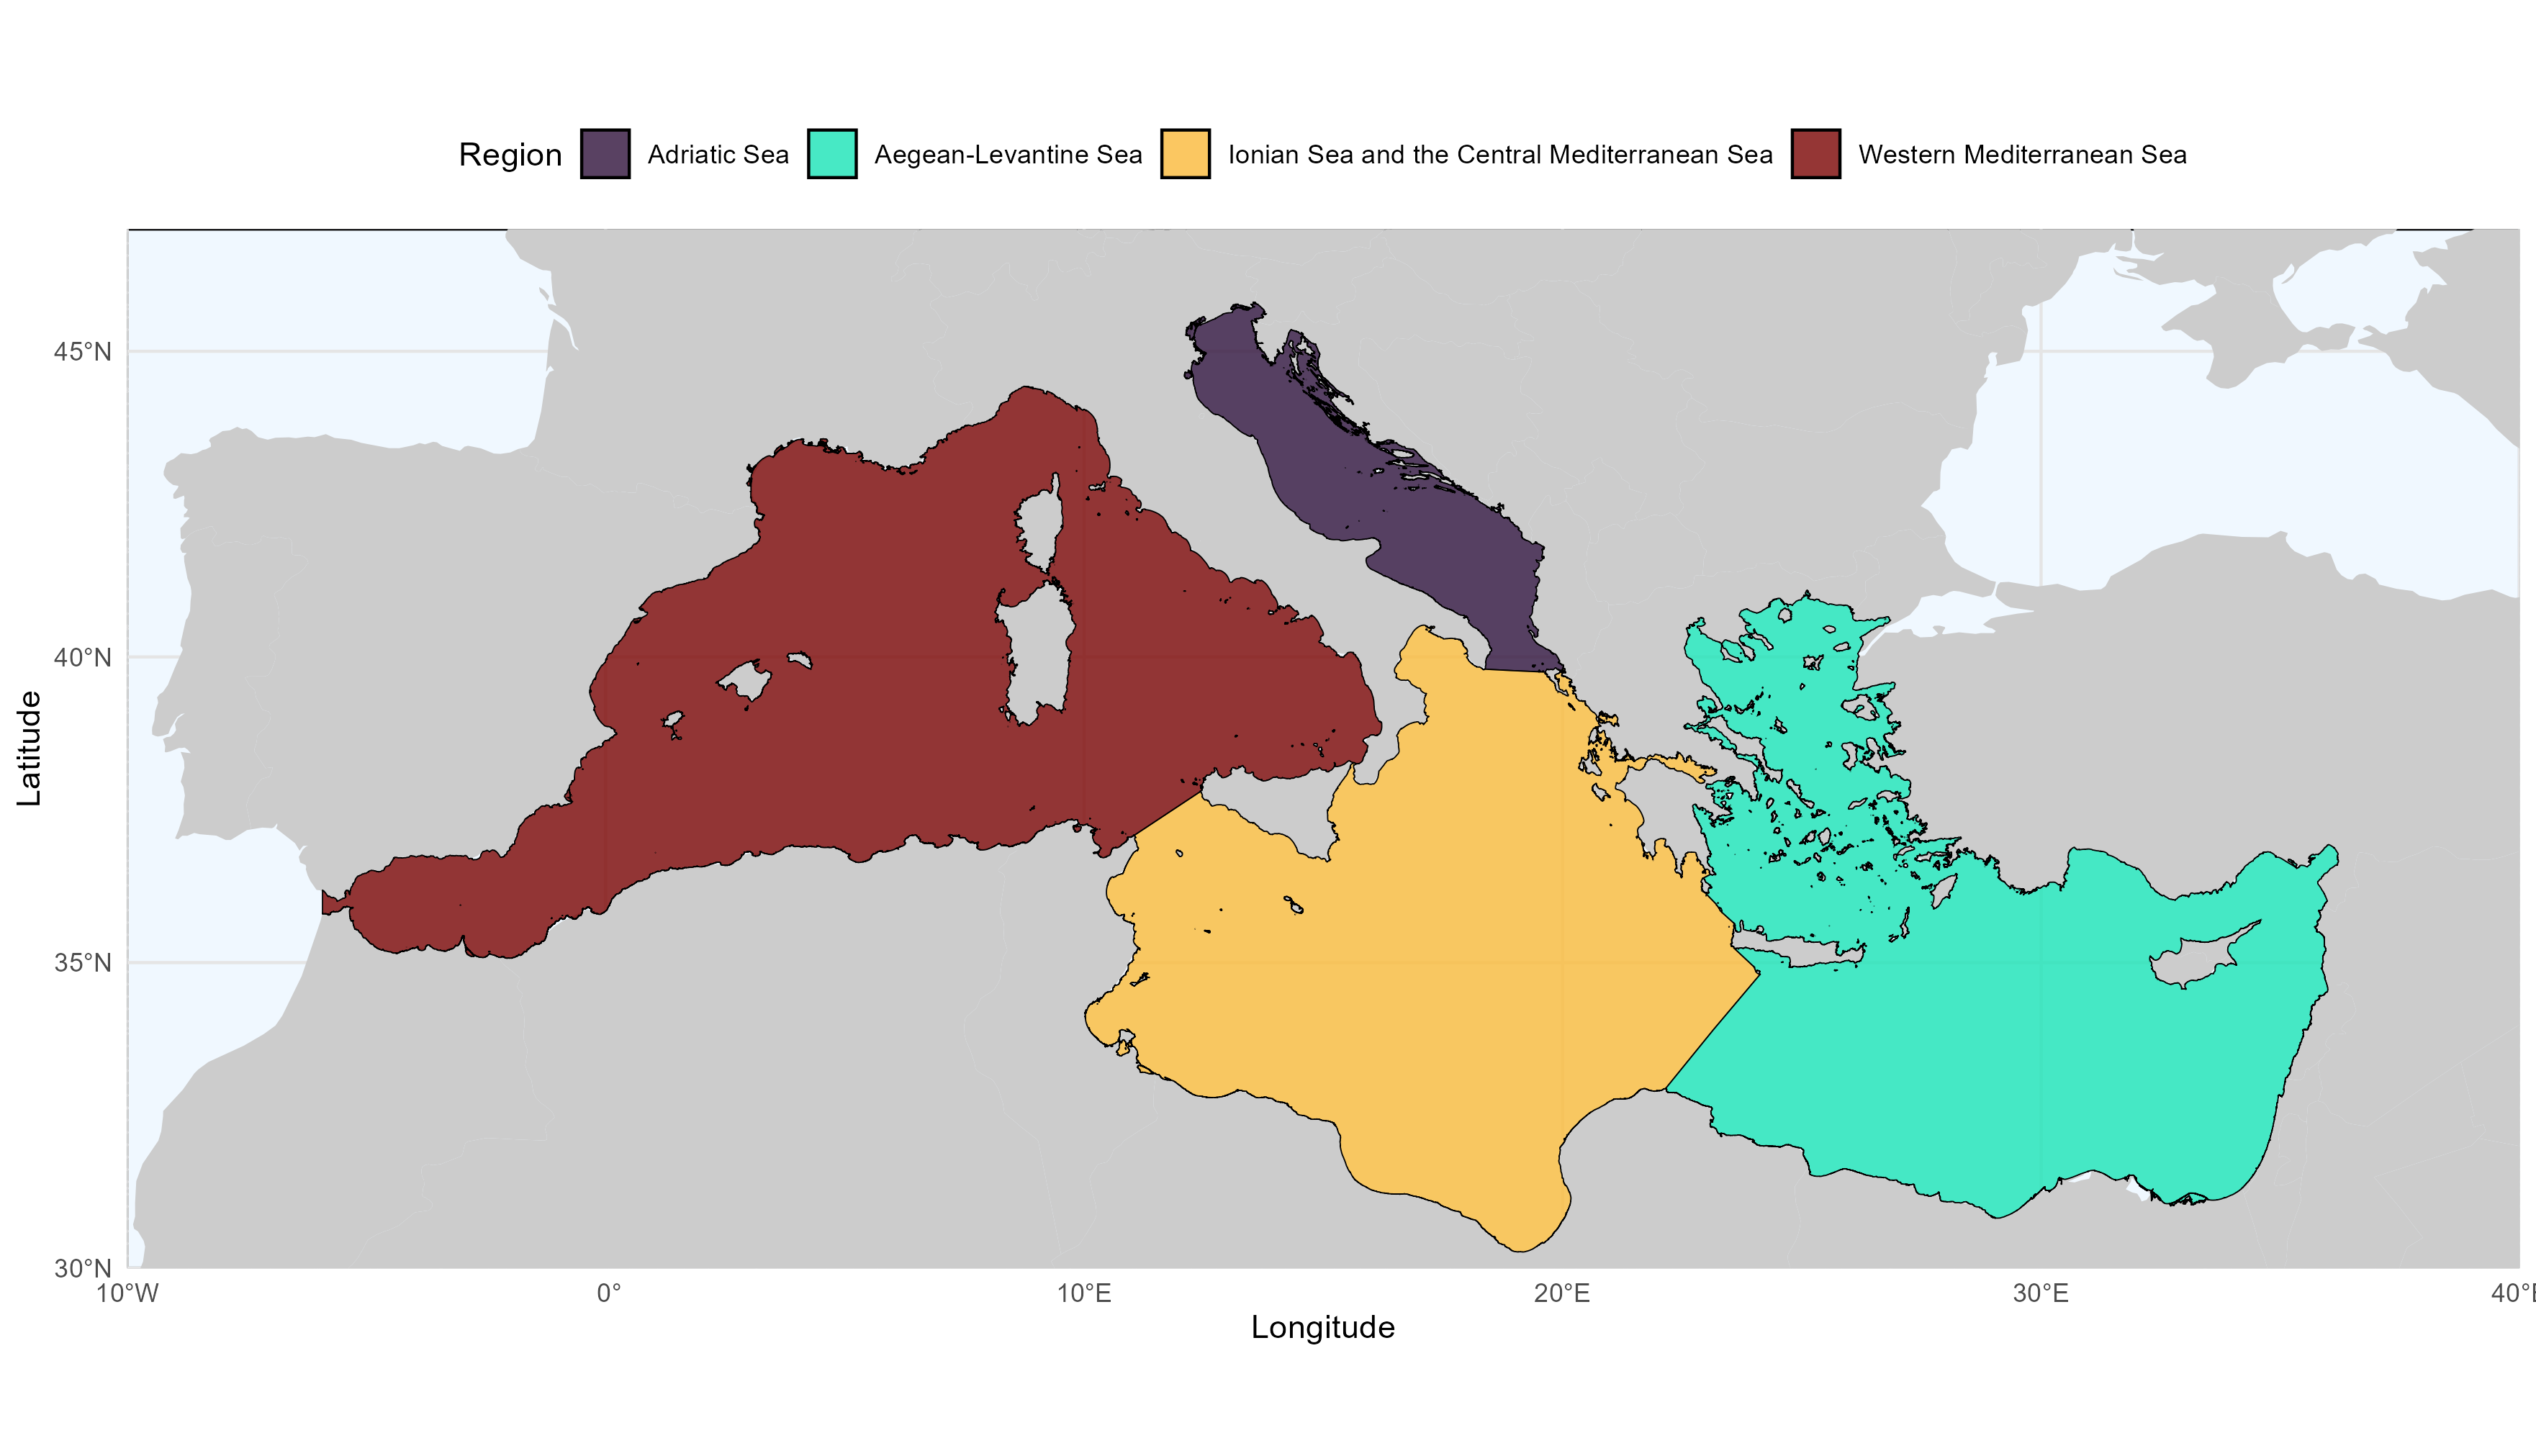
\includegraphics[width=1\linewidth,height=\textheight,keepaspectratio]{Figs/Map_MedSea.png}

}

\caption{\label{fig-MapMedSea}Region of Mediterranean Sea as definied by
Marine Strategy Framework Directive.}

\end{figure}%


\bibliography{library.bib}



\end{document}
